% =================================================================
\documentclass[ 10pt, xcolor = dvipsnames]{beamer}
\usepackage{ beamerthemesplit, lmodern}
\usetheme{Madrid}
\usecolortheme[named=Brown]{structure}
\useinnertheme{rectangles}
\setbeamertemplate{frametitle continuation}{}
\beamertemplatenavigationsymbolsempty
\usepackage{../../macros-general}
\usepackage{../../macros-beamer}
\graphicspath{{./figures/}}

\newcommand{\theoremblock}[2]{
\begin{center}
\begin{minipage}{0.9\columnwidth}
\begin{block}{#1}
#2
\end{block}
\end{minipage}
\end{center}
}
\newcommand{\Laplace}{\mathcal{L}}
\newcommand{\LaplaceInv}{\Laplace^{-1}}

% =================================================================
\newcommand{\shorttitle}{Control Systems Engineering - Unit 03}
\title[\shorttitle]{Control Systems Engineering (EYAG-1005): \\ \textbf{Unit 03} }
\author[L. I. Reyes-Castro]{Luis I. Reyes-Castro}
\institute[ESPOL]{\normalsize Escuela Superior Polit\'ecnica del Litoral (ESPOL) \\ Guayaquil - Ecuador}
\date[2017-T1]{Semester: 2017-T1}

% -----------------------------------------------------------------
\begin{document}
\begin{frame}[noframenumbering]
\titlepage
\end{frame}
\begin{frame}[noframenumbering]
\frametitle{\shorttitle}
\tableofcontents[ subsectionstyle = hide]
\end{frame}

\AtBeginSection[]
{
\begin{frame}
\frametitle{Contenido del Tema}
\tableofcontents[ currentsection, sectionstyle = show/shaded, subsectionstyle = show/show/hide]
\end{frame}
}
\AtBeginSubsection[]
{
\begin{frame}
\frametitle{Contenido del Tema}
\tableofcontents[ currentsection, currentsubsection, sectionstyle = show/shaded, subsectionstyle = show/shaded/hide]
\end{frame}
}


% =================================================================
\section{First-order Systems}

% -----------------------------------------------------------------
\begin{frame}[allowframebreaks]
\frametitle{\insertsection}

\textbf{Definition:}

We say that a system with transfer function $G(s)$ is of first-order if: 
\[
G(s) \; = \; \frac{K}{ s + \sigma }
\qquad \text{for some } K, \sigma > 0
\]
\framebreak

Step response, \ie $r(t) \, = \, u(t)$ : 
\begin{align*}
R(s) \; = \; \frac{1}{s} \qquad 
& \Longrightarrow \quad
c(t) \; = \; \LaplaceInv[ \, R(s) \, G(s) \, ] \\
& \Longrightarrow \quad
c(t) \; = \; \LaplaceInv \left[ \;
\frac{K}{ s ( s + \sigma ) } \; \right] \\[2ex]
& \Longrightarrow \quad
c(t) \; = \; \LaplaceInv \left[ \;
\frac{K / \sigma}{s} - \frac{K / \sigma}{s + \sigma} \; \right] \\[2ex]
& \Longrightarrow \quad
c(t) \; = \; \left[ \;
\frac{K}{\sigma} - \frac{K}{\sigma} \, e^{ -\sigma t }
\; \right] u(t) \, , \quad \forall t \in \Re \\[2ex]
& \Longrightarrow \quad
c(t) \; = \; 
\frac{K}{\sigma} - \frac{K}{\sigma} \, e^{ -\sigma t },
\quad \forall t \geq 0
\end{align*}

\end{frame}

%% =================================================================
\section{Second-order Systems}

% -----------------------------------------------------------------
\begin{frame}[allowframebreaks]
\frametitle{\insertsection}

Recall the following results from elementary algebra: 
\begin{itemize}
\item For any $\alpha, \beta, \gamma \in \Re$ the roots of the second-order polinomial 
\[
D(s) \, = \, \alpha \, s^2 + \beta \, s + \gamma
\]
are as follows:  
\[
s_1 \; = \; 
-\frac{\beta}{2 \alpha} + \frac{\sqrt{ \beta^2 - 4 \, \alpha \, \gamma }}{2 \, \alpha} \qquad \qquad
s_2 \; = \; 
-\frac{\beta}{2 \alpha} + \frac{\sqrt{ \beta^2 - 4 \, \alpha \, \gamma }}{2 \, \alpha}
\]
Therefore: 
\begin{itemize}
\item If $\beta^2 > 4 \, \alpha \, \gamma$ then the roots are repeated and different. 
\item If $\beta^2 = 4 \, \alpha \, \gamma$ then the roots are repeated and identical. 
\item If $\beta^2 < 4 \, \alpha \, \gamma$ then the roots are complex conjugates. 
\end{itemize}
\framebreak

\item For any $a, b \in \Re$ the roots of the second-order polinomial 
\[
D(s) \, = \, s^2 + a \, s + b
\]
are as follows:  
\[
s_1 \; = \; 
-\frac{a}{2} + \frac{\sqrt{ a^2 - 4b }}{2} \qquad \qquad
s_2 \; = \; 
-\frac{a}{2} - \frac{\sqrt{ a^2 - 4b }}{2}
\]
Therefore: 
\begin{itemize}
\item If $a^2 > 4 b$ then the roots are repeated and different. 
\item If $a^2 = 4 b$ then the roots are repeated and identical. 
\item If $a^2 < 4 b$ then the roots are complex conjugates. 
\end{itemize}

\end{itemize}

\end{frame}

%% =================================================================
%\section{Stability}

% =================================================================
\section{Steady-state Errors}

% -----------------------------------------------------------------
\begin{frame}[allowframebreaks]
\frametitle{\insertsection}

Recall the reference signals: 
\begin{figure}
\centering
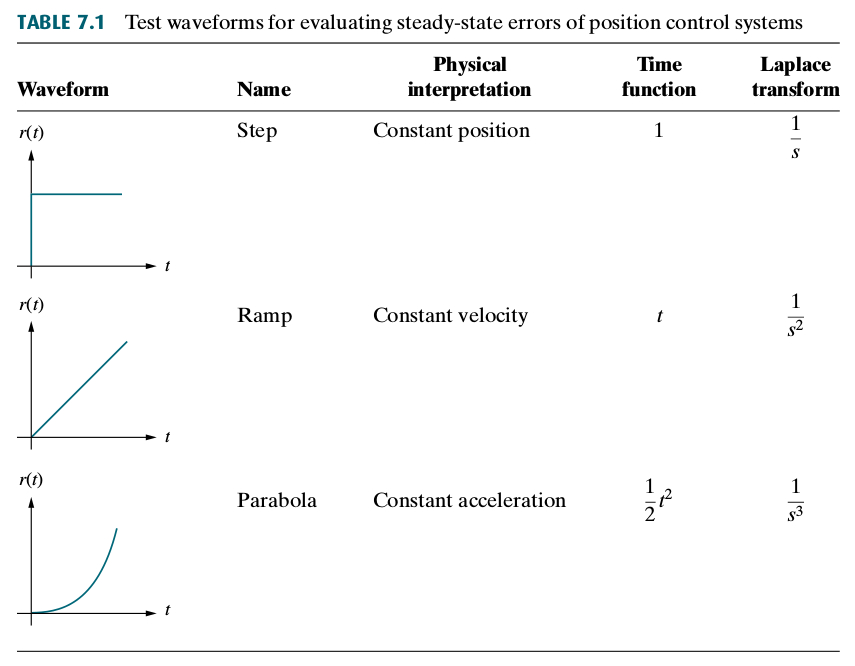
\includegraphics[width=0.72\columnwidth]{figures/Nise_Table-7-1.jpg}
\end{figure}
\framebreak

Recall the following property of the Laplace Transform: 

\theoremblock{Final Value Theorem}{
For any function $f(t)$ defined for $t \geq 0$ with Laplace Transform $F(s)$ \linebreak we have that: 
\[
\lim_{ t \rightarrow \infty } \, f(t) \quad = \quad
\lim_{ s \rightarrow 0 } \, s \, F(s)
\]
\halfskip
}

\end{frame}

% -----------------------------------------------------------------
\begin{frame}[allowframebreaks]
\frametitle{\insertsection}

Steady-state errors for simple feedthrough systems: 
\fullskip

\begin{figure}
\centering
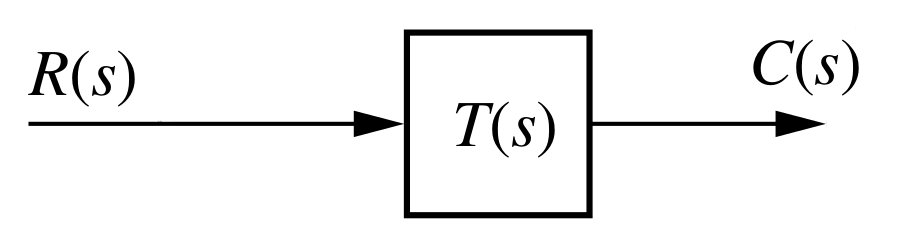
\includegraphics[width=0.4\columnwidth]{figures/Nise_Fig-7-3a.jpg}
\end{figure}
\begin{align*}
& E(s) \; = \; R(s) - C(s) \; = \; R(s) - T(s) \, R(s) \\[1ex]
& \Longrightarrow \; E(s) \; = \; R(s) \, [ \, 1 - T(s) \, ] \\[1ex]
& \Longrightarrow \; e(\infty) \; = \; 
\lim_{ t \rightarrow \infty } e(t) \; = \; 
\lim_{ s \rightarrow 0 } s \, E(t) \; = \; 
\lim_{ s \rightarrow 0 } \; s \, R(s) \, [ \, 1 - T(s) \, ]
\end{align*}
\framebreak

\begin{itemize}
\item Step input $r(t) \, = \, u(t)$ :
\[
R(s) \, = \, \frac{1}{s} \qquad \Longrightarrow \qquad
e_{step}(\infty) \; = \; 
\lim_{ s \rightarrow 0 } \; 1 - T(s)
\]
\item Ramp input $r(t) \, = \, t \, u(t)$ :
\[
R(s) \, = \, \frac{1}{s^2} \qquad \Longrightarrow \qquad
e_{ramp}(\infty) \; = \; 
\lim_{ s \rightarrow 0 } \; \frac{1 - T(s)}{s}
\]
\item Parabolic input $r(t) \, = \, (1/2) \, t^2 \, u(t)$ :
\[
R(s) \, = \, \frac{1}{s^3} \qquad \Longrightarrow \qquad
e_{parabolic}(\infty) \; = \; 
\lim_{ s \rightarrow 0 } \; \frac{1 - T(s)}{s^2}
\]
\end{itemize}

\end{frame}

% -----------------------------------------------------------------
\begin{frame}[allowframebreaks]
\frametitle{\insertsection}

Steady-state errors for unity-feedback systems: 
\fullskip

\begin{figure}
\centering
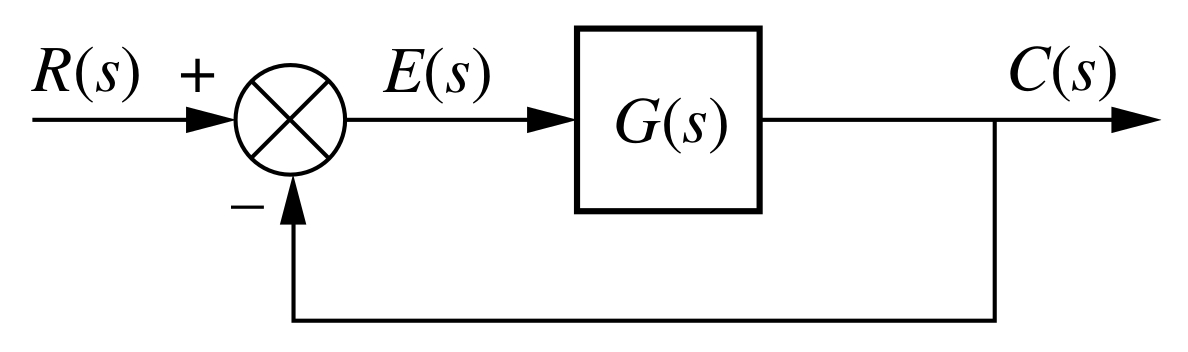
\includegraphics[width=0.5\columnwidth]{figures/Nise_Fig-7-3b.jpg}
\end{figure}
\begin{align*}
& E(s) \; = \; R(s) - C(s) \; = \; R(s) - G(s) \, E(s) \\[1ex]
& \Longrightarrow \; E(s) \, [ \, 1 + G(s) \, ] \; = \; R(s) \\[1ex]
& \Longrightarrow \; E(s) \; = \; \frac{R(s)}{1 + G(s)} \\[1ex]
& \Longrightarrow \; e(\infty) \; = \; 
\lim_{ t \rightarrow \infty } e(t) \; = \; 
\lim_{ s \rightarrow 0 } s \, E(t) \; = \; 
\lim_{ s \rightarrow 0 } \; \frac{ s \, R(s) }{1 + G(s)}
\end{align*}
\framebreak

\begin{itemize}
\item Step input $r(t) \, = \, u(t)$ :
\[
R(s) \, = \, \frac{1}{s} \qquad \Longrightarrow \qquad
e_{step}(\infty) \; = \; 
\lim_{ s \rightarrow 0 } \; \frac{1}{1 + G(s)}
\]
\item Ramp input $r(t) \, = \, t \, u(t)$ :
\[
R(s) \, = \, \frac{1}{s^2} \qquad \Longrightarrow \qquad
e_{ramp}(\infty) \; = \; 
\lim_{ s \rightarrow 0 } \; \frac{1}{s \, G(s)}
\]
\item Parabolic input $r(t) \, = \, (1/2) \, t^2 \, u(t)$ :
\[
R(s) \, = \, \frac{1}{s^3} \qquad \Longrightarrow \qquad
e_{parabolic}(\infty) \; = \; 
\lim_{ s \rightarrow 0 } \; \frac{1}{s^2 \, G(s)}
\]
\end{itemize}

\end{frame}

% -----------------------------------------------------------------
\begin{frame}[allowframebreaks]
\frametitle{\insertsection}

Furthermore, for unity-feedback systems: 
\begin{itemize}
\item Position constant $K_p$ :
\[
K_p \; = \; \lim_{ s \rightarrow 0 } \; G(s)
\qquad \Longrightarrow \qquad
e_{step}(\infty) \; = \; \frac{1}{1 + K_p}
\]
\item Velocity constant $K_v$ :
\[
K_v \; = \; \lim_{ s \rightarrow 0 } \; s \,G(s)
\qquad \Longrightarrow \qquad
e_{ramp}(\infty) \; = \; \frac{1}{K_v}
\]
\item Acceleration constant $K_a$ :
\[
K_a \; = \; \lim_{ s \rightarrow 0 } \; s^2 \,G(s)
\qquad \Longrightarrow \qquad
e_{parabolic}(\infty) \; = \; \frac{1}{K_a}
\]
\end{itemize}

\end{frame}

% -----------------------------------------------------------------
\begin{frame}[allowframebreaks]
\frametitle{\insertsection}

\textbf{System Type:}
Number of integrators (poles at $s = 0$) on the forward path.

\begin{figure}
\centering
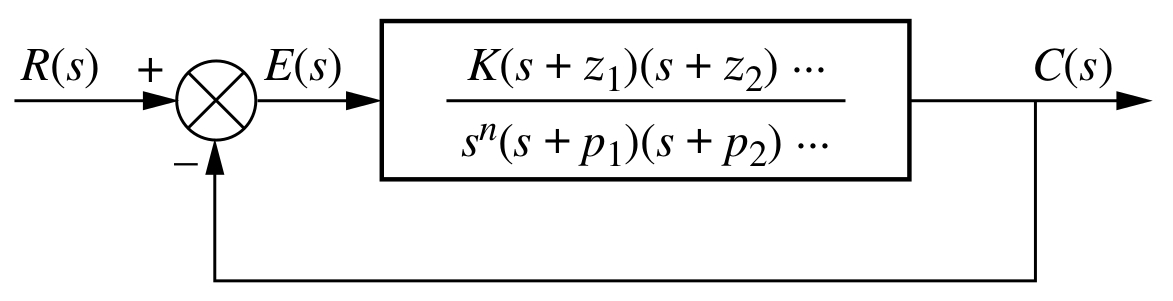
\includegraphics[width=0.6\columnwidth]{figures/Nise_Fig-7-8.jpg}
\end{figure}
\fullskip

Steady-state error as a function of system type:
\begin{figure}
\centering
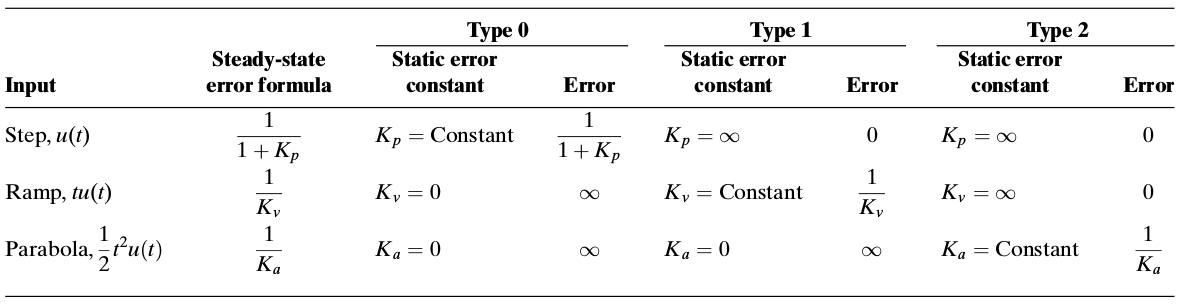
\includegraphics[width=\columnwidth]{figures/Nise_Table-7-2.jpg}
\end{figure}

\end{frame}

% -----------------------------------------------------------------
\begin{frame}[allowframebreaks]
\frametitle{\insertsection}

For non-unity non-unity-feedback systems, simply re-write the system in unity-feedback form: 
\fullskip

\begin{figure}
\centering
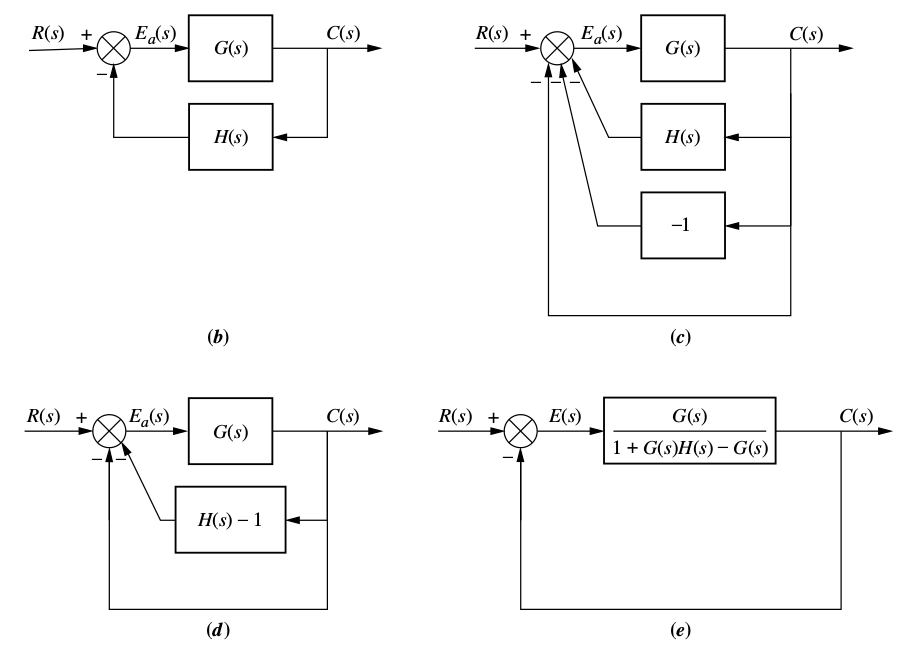
\includegraphics[width=0.7\columnwidth]{figures/Nise_Fig-7-15.jpg}
\end{figure}

\end{frame}

% =================================================================
\section{Evan's Root Locus}

% -----------------------------------------------------------------
\begin{frame}[allowframebreaks]
\frametitle{\insertsection}

Motivating example: 
\fullskip

\begin{figure}
\centering
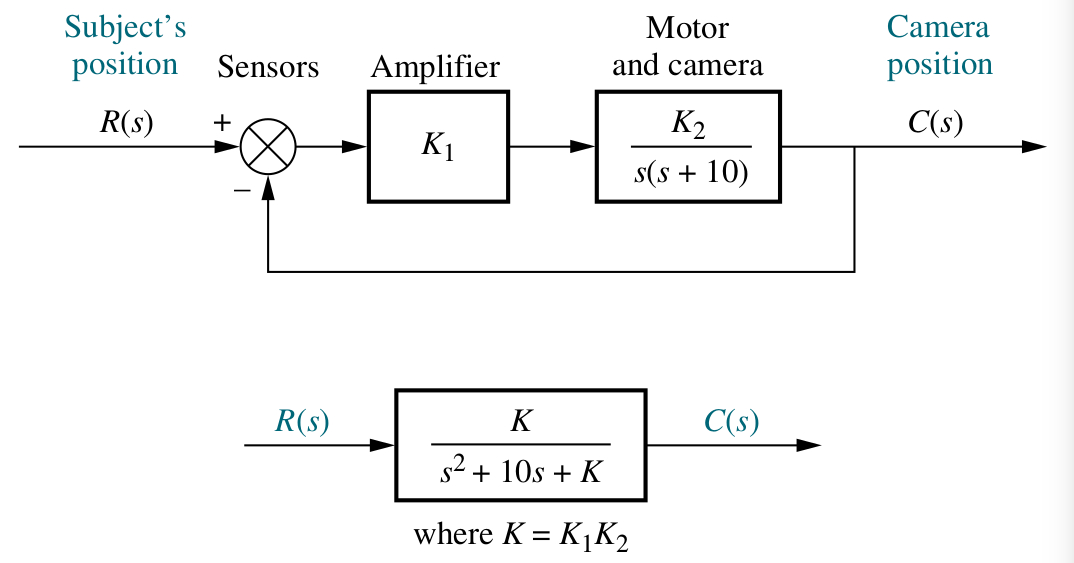
\includegraphics[width=0.68\columnwidth]{figures/Nise_Figure-8-4.jpg}
\end{figure}
\framebreak

\begin{figure}
\centering
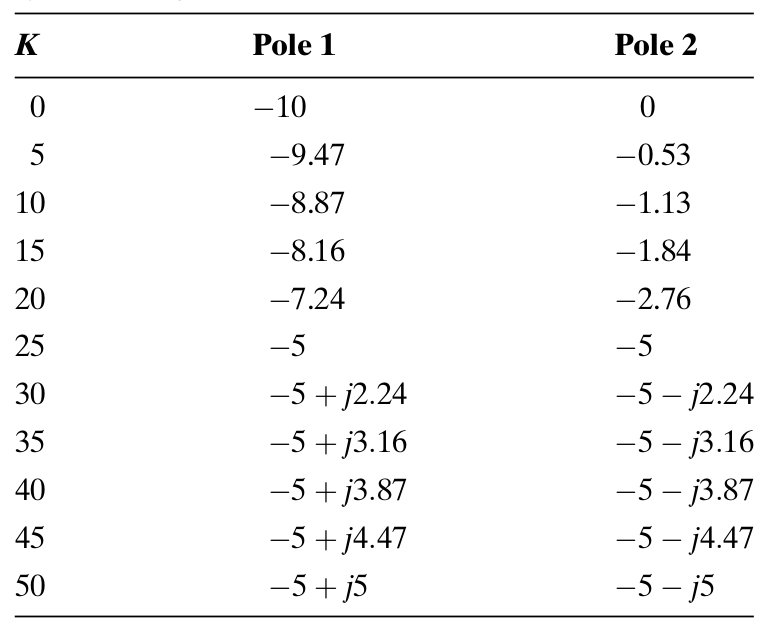
\includegraphics[width=0.56\columnwidth]{figures/Nise_Table-8-1.jpg}
\end{figure}

\end{frame}

% -----------------------------------------------------------------
\begin{frame}[allowframebreaks]
\frametitle{\insertsection}

The root locus concerns the design of closed-loop control systems with the following architecture: 
\begin{figure}
\centering
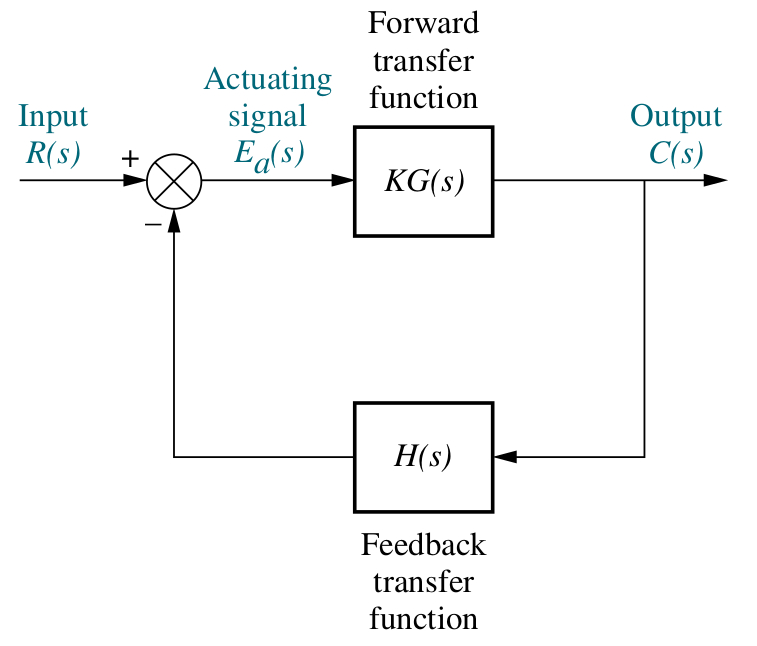
\includegraphics[width=0.5\columnwidth]{figures/Nise_Figure-8-1.jpg}
\end{figure}
\framebreak

Definitions: 
\begin{itemize}
\item Loop gain: $K$
\item Open-loop transfer function: $G(s) \, H(s)$
\end{itemize}
\fullskip

Objective: 
\begin{itemize}
\item Sketch the roots of the closed-loop transfer function as the loop gain $K$ \linebreak ranges from near zero (\ie $K \rightarrow 0^+$) to infinity (\ie $K \rightarrow +\infty$). 
\end{itemize}

\end{frame}

% -----------------------------------------------------------------
\begin{frame}[allowframebreaks]
\frametitle{\insertsection}

Root locus sketching rules:
\begin{itemize}
\item The root locus is symmetric about the real axis. 
\item The number of branches, \ie pole trayectories, equals the number of poles \linebreak of the open-loop transfer function. 
\item Each branch begins at an open-loop pole and ends either: 
\begin{itemize}
\item At an open-loop zero. 
\item At infinity along an asymptote. 
\end{itemize}
\item Along the real line, root locus branches can be found to the left of any \linebreak odd number of real open-loop poles or open-loop zeros. 
\framebreak

\item If the root locus has asymptotes, then the number of asymptotes is: 
\[
\text{ ( number of open-loop poles ) } -  
\text{ ( number of open-loop zeros ) }
\]
%\fullcut
%\begin{itemize}
%\item This assumes, of course, that $G(s)$ is a \emph{causal} transfer function, \ie that \linebreak the order of its numerator does not exceed the order of its denominator. 
%\end{itemize}
\item If the root locus has asymptotes, then the centroid of the asymptotes is located along the real axis at the point: 
\[
\sigma_a \; = \; 
\frac{ \sum \text{(open-loop pole locations)} - \sum \text{(open-loop zero locations)} }{ \text{number of asymptotes} }
\]
\item If the root locus has asymptotes, then their angles in radians are: 
\[
\theta_a \; = \; 
\frac{ ( 2k + 1 ) \, \pi }{ \text{number of asymptotes} }
\qquad
\text{for } k \, = \, 0, \, \pm 1, \, \pm 2, \, \dots
\]
\end{itemize}

\end{frame}

% =================================================================
\section{Bode Plots}

% -----------------------------------------------------------------
\begin{frame}[allowframebreaks]
\frametitle{\insertsection}

Consider a stable system with transfer function $G(s)$. 
\begin{itemize}
\item Suppose the input $r(t)$ is a sinusoid with frequency $\omega$ and unit amplitude. 
\item Then the steady-state output $c_{ss}(t)$ must be a a sinusoid with the same frequency $\omega$ but with a particular amplitude $M$ and phase $\phi$ which depend \linebreak on the transfer function $G(s)$ and on the input frequency $\omega$. 
\end{itemize}
\halfskip

\begin{figure}[htb]
\centering
\def\svgwidth{0.8\columnwidth}
\input{figures/Bode-plot_definition.eps_tex}
\end{figure}
\framebreak

\begin{itemize}
\item Given $G(s)$ and a frequency $\omega$ we can evaluate the amplitude and phase of the steady-state output by computing the phasor $G(j\omega)$. In particular: 
\begin{itemize}
\item The phasor's magnitude yields the amplitude $M(\omega)$. 
\item The phasor's angle with $+\Re$ yields the phase $\phi(\omega)$. 
\end{itemize}
\halfskip
\begin{figure}[htb]
\centering
\def\svgwidth{0.72\columnwidth}
\input{figures/Bode-plot_phasor.eps_tex}
\end{figure}

\end{itemize}
\framebreak

\begin{itemize}
\item We can also estimate $M(\omega)$ and $\phi(\omega)$ experimentally: 
\halfskip
\begin{figure}[htb]
\centering
\def\svgwidth{0.8\columnwidth}
\input{figures/Bode-plot_sinewaves.eps_tex}
\end{figure}
\end{itemize}
\framebreak

\begin{itemize}
\item Furthermore, notice that: 
\begin{itemize}
\item Amplitude $M$ is always positive. 
\begin{itemize}
\item If $M \in (0,1)$ we get attenuation. 
\item If $M = 1$ we get amplitude matching. 
\item If $M > 1$ we get amplification. 
\end{itemize}
\item Phase may be negative, zero or postive. 
\begin{itemize}
\item If $\phi < 0$ then the output lags the input. 
\item If $\phi = 0$ then the output matches the input. 
\item If $\phi > 0$ then the output leads the input. 
\end{itemize}
\end{itemize}
\end{itemize}

\end{frame}

% -----------------------------------------------------------------
\begin{frame}[allowframebreaks]
\frametitle{\insertsection}

\textbf{Bode Plots} are diagrams of $M(\omega)$ and $\phi(\omega)$. More precisely, they consist of \linebreak the following two plots: 
\begin{itemize}
\item \textbf{Magnitude Plot}: Amplitude $M(\omega)$ versus frequency $\omega$. 
\begin{itemize}
\item The $x$-axis is frequency $\omega$ in decades, \ie $x = \log_{10}(\omega)$. 
\item The $y$-axis is amplitude $M(\omega)$ in decibels, \ie $y = 20 \cdot \log(M(\omega))$. 
\end{itemize}
\item \textbf{Phase Plot}: Phase $\phi(\omega)$ versus frequency $\omega$. 
\begin{itemize}
\item The $x$-axis is frequency $\omega$ in decades, \ie $x = \log_{10}(\omega)$. 
\item The $y$-axis is phase in degrees, \ie $y = \phi(\omega)$. 
\end{itemize}
\end{itemize}
\halfskip

Notice that when sketching Bode Plots by hand, we usually don't draw exactly \linebreak the functions $M(\omega)$ and $\phi(\omega)$ but instead sketch \emph{asymptotic approximations}. 

\end{frame}

% -----------------------------------------------------------------
\begin{frame}[allowframebreaks]
\frametitle{\insertsection}

Bode plot for a simple amplifier: $G(s) = K$
\begin{itemize}
\item Magnitude plot is constant at $y = 20 \cdot \log_{10}(K)$ decibels. 
\item Phase plot is constant at $y = 0$ degree. 
\end{itemize}
\framebreak

Bode plot for an integrator: $\displaystyle G(s) = \frac{1}{s}$
\begin{itemize}
\item Phasor as a function of $\omega$ : 
\[
G(j\omega) \; = \; \frac{1}{j\omega} \; = \; -\frac{j}{\omega} 
\qquad \Longrightarrow \qquad
M(\omega) \; = \; \frac{1}{\omega} \quad \& \quad
\phi(\omega) \; = \; -90^{\circ}
\]
\item Magnitude plot is $y = -20 \cdot \log_{10}(\omega)$ decibels, \ie it is a line with slope of $-20$ decibels per decade which hits zero decibels at $\omega = 1$ rad/s. 
\item Phase plot is constant at $y = -90$ degree. 
\end{itemize}
\framebreak

Bode plot for a differentiator: $\displaystyle G(s) = s$
\begin{itemize}
\item Phasor as a function of $\omega$ : 
\[
G(j\omega) \; = \; j\omega \qquad \Longrightarrow \qquad
M(\omega) \; = \; \omega \quad \& \quad
\phi(\omega) \; = \; +90^{\circ}
\]
\item Magnitude plot is $y = +20 \cdot \log_{10}(\omega)$ decibels, \ie it is a line with slope of $+20$ decibels per decade which hits zero decibels at $\omega = 1$ rad/s. 
\item Phase plot is constant at $y = +90$ degree. 
\end{itemize}

\end{frame}

\end{document}
